\documentclass{book}

\usepackage{tikz}
\usepackage{tikz-3dplot}
\usepackage{pgfplots}

\pagestyle{empty}

\begin{document}
% sqare of half axes

\newcommand{\asa}{2}
\newcommand{\bsa}{0.5}
\newcommand{\csa}{0.4}

% view angle
\tdplotsetmaincoords{70}{135}

\begin{tikzpicture}[scale=2,tdplot_main_coords,line join=bevel,fill opacity=.8]
    \pgfsetlinewidth{.1pt}
    \tdplotsphericalsurfaceplot[parametricfill]{72}{36}%
        {1/sqrt((sin(\tdplottheta))^2*(cos(\tdplotphi))^2/\asa+
        (sin(\tdplottheta))^2*(sin(\tdplotphi))^2/\bsa + (cos(\tdplottheta))^2/\csa)} % function defining radius
        {black!20} % line color
        {2*\tdplottheta} % fill
        {\draw[color=black,thick,->] (0,0,0) -- (2,0,0) node[anchor=north east]{$x$};}% x-axis
        {\draw[color=black,thick,->] (0,0,0) -- (0,1.5,0) node[anchor=north west]{$y$};}% y-axis
        {\draw[color=black,thick,->] (0,0,0) -- (0,0,1) node[anchor=south]{$z$};}% z-axis
\end{tikzpicture}

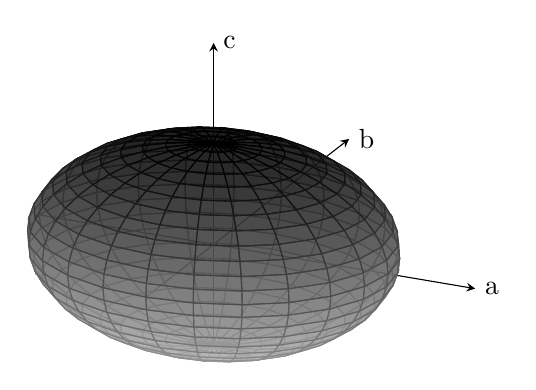
\begin{tikzpicture}
    \begin{axis}[%
        width=0.8\textwidth,
        %axis equal,
        axis lines = center,
        x label style={at={(axis cs:3,0,0)},anchor=west},
        y label style={at={(axis cs:0,4,0)},anchor=west},
        z label style={at={(axis cs:0,0,1)},anchor=west},
        xlabel = {a},
        ylabel = {b},
        zlabel = {c},
        xmax=3,
        ymax=4,
        zmax=1,
        ticks=none,
        colormap={}{ gray(0cm)=(0.8); gray(1cm)=(0);}
    ]
    \addplot3[%
        fill opacity=0.7,
        surf,
		% I don't think the shaders improve the plot, so I left them commented out.
		% Feel free to play with them. Same holds true for the increased number of samples.
                %shader=flat,
                %shader=interp,
                %shader=faceted,
                %shader=flat corner,
                %shader=flat mean,
                %shader=faceted interp,
                %samples = 50,
                domain=0:2*pi,y domain=0:pi,
                z buffer=sort
                ]
                ({2*cos(deg(x))*sin(deg(y))}, {2*sin(deg(x))*sin(deg(y))}, {0.5*cos(deg(y))});
    \end{axis}

\end{tikzpicture}

\end{document}
